%
% File: chap01.tex
%
\let\textcircled=\pgftextcircled
\chapter{Theory}
\label{chap:intro}

\initial{A} very valuable measurement obtained from a reactor core is the neutron flux. Its computation allow the iperator to know what the core and fuel elements are subjected to, in terms of local power peak, temperature and irradiation. In a reactor such as the GSTR, used mainly for sample irradiation, knowing the flux seen by the samples in the different testing tubes is very important. This allows for the irradiation to be done for an adequate period of time. Neutron detectors can give a good idea of the overall flux in the core, but are oblivious to local effects. The theory is based off of the course material~\cite{debey01}.

\section{Target selection}

The sample to be irradiated needs to be chosen carefully. The choice depends on the threshold energy, the corresponding cross section of the element and its half-life. Table~\ref{tab:target} presents potential elments that could be used for thermal flux monitoring.

\begin{table}[t]
\centering
\caption{Foil element characteristics after irradiation}
\label{tab:target}
\begin{tabular}{|c|c|c|c|c|}
\hline
Foil Element & Reaction      & Threshold energy (keV) & Cross-section (b) & Half-life \\ \hline\hline
Gold         & (n, $\gamma$) & thermal                & 98.8              & 2.69d     \\ \hline
Aluminium    & (n, $\gamma$) & thermal                & 0.23              & 2.3m      \\ \hline
Dysprosium   & (n, $\gamma$) & thermal                & 920               & 139m      \\ \hline
Sodium       & (n, $\gamma$) & thermal                & 0.53              & 15h       \\ \hline
\end{tabular}
\end{table}

Gold is an obvious candidate, its high cross-section allowing for lower concentrations and its half-life being long enough to give the operator some time, and potentially do several measurements over the course of a week to confirm the results. The half-life is also short enough that after a month, the sample would be back to its normal activation state. Aluminium use in a neutron flux monitoring case is limited by its short half-life. The samples activation would have to be measured in an unrealistically constrained time. Dysprosium presents a very high cross-section and a reasonable half-life. All things considered, for our experiment, Sodium is an obvious choice, due to its abundance in high purity form and its 15 hours half-life.

NaCl compound, used in this project, can be obtained at high purity at low cost. The other activated isotopes created by irradiation of Sodium present either a very short ($F_{20}$, few seconds) or fairly high ($Na_{22}$, several years) half-life, thus not compromising the results from the spectrometry.

\section{Target activation}

In order to compute the irradiation time needed as well as the decay time to apply to the sample, one can use equation~\ref{eq:act}. This equation gives the sample activation given a theorized flux after the irradiation of the sample in the core during t. It can then be plugged into equation~\ref{eq:decay} in order to compute the expected sample activation after a decay time T.

\begin{equation}
A_0 = \sigma\phi\frac{m}{A}\frac{N_A}{c}(1-e^{-\lambda t})
\label{eq:act}
\end{equation}
Where:
\begin{conditions}
A_0 & Activity at the end of the irradiation ($Ci$) \\
\sigma & Microscopic neutron cross-section ($cm^2$) \\
\phi & Neutron flux ($n.cm^{-2}.s^{-1}$) \\
m & Mass of the target isotope ($g$) \\
A & Atomic weight of the target isotope \\
\lambda & Decay constant of the radionuclide ($s^{-1}$) \\
t & Irradiation time ($s$) \\
N_A & Avogadro constant \\
c & Conversion factor from number of disintegrations per second to Curies : $3.7 * 10^{10}$
\end{conditions}

\begin{equation}
A_1 = A_0 e^{-\lambda T}
\label{eq:decay}
\end{equation}
Where:
\begin{conditions}
A_1 & Activity at the end of the decay period ($Ci$) \\
T & Decay time after irradiation ($s$)
\end{conditions}

In the case of the NaCl compound considered, Table~\ref{tab:nacl} gives the intermediate calculation steps. It considers that Chlorine-38 represents 25\% of the total Chlorine activated, the other 75\% being considered stable (half-life around 300000 years). A mass of 0.4 mg of NaCl compound is considered. Considering a neutron flux estimated at $10^{13}\ n.cm^{-2}.s^{-1}$ within the central thimble, and an irradiation time of five minutes, the activity estimated right after the five minutes irradiation is 2.27 $\micro Ci$ for the Sodium, and 879 $\micro Ci$ for the Chlorine. Figure~\ref{fig:dec} presents the activity change with time during the decay period. A decay time of around 24 hours was chosen. It can be noted that the activity provided by the Chlorine-38 disappears almost completely after 10 half-life, around 6 hours.

\begin{table}[t]
\centering
\caption{Specific data for NaCl compound}
\label{tab:nacl}
\begin{tabular}{|l|c|c|}
\hline
NaCl               & $Na_{24}$      & $Cl_{38}$       \\ \hline
$\sigma \ (cm^{-2})$ & $5.3*10^{-25}$ & $3.55*10^{-23}$ \\ \hline
$m\ (g)$            & $1.57*10^{-4}$ & $6.07*10^{-5}$  \\ \hline
$A$                & 22.9898        & 35.453          \\ \hline
$\lambda \ (s^{-1})$ & $1.28*10^{-5}$ & $3.10*10^{-4}$  \\ \hline
\end{tabular}
\end{table}

\begin{figure}[t!]
	\centering
	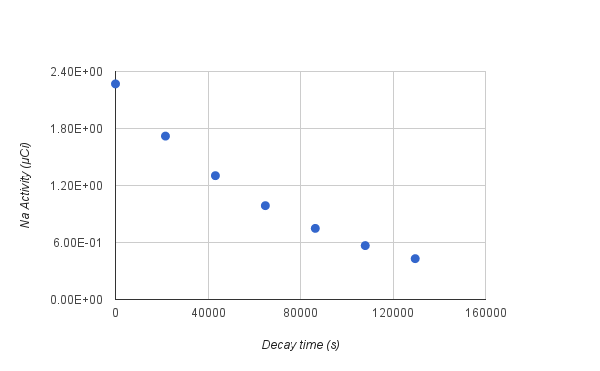
\includegraphics[height=0.4\textheight]{fig01/decay.png}
	\mycaption[Activity of the sample after irradiation]{Activity of the sample after irradiation.}
	\label{fig:dec}
\end{figure}

The experiment will consequently measure the activation from samples of 0.4 mg of NaCl placed over a 20 cm distance in the core. It is expected, if the flux estimates of $10^{13}\ n.cm^{-2}.s^{-1}$ is correct, to obtain an activity of around 0.7 $\micro Ci$ during the spectrometry data experiments, a day after the irradiation.

It is interesting to note that starting after around five half-lives of irradation time, the sample can be considered irradiated at saturation. This means that the equilibrium between the buildup of radioisotopes through irradiation and the decay of those isotopes in the sample has been reached. At this point, the sample activity will reach a plateau. In the case of our experiment, the sample will not be anywhere near saturation levels, since this would imply an irradiation time greater than three days.

\section{Spectrometry}
The samples activities are measured using a spectrometer. A more detailed explanation of the spectrometer use can be found in a previous report~\cite{glher01}.


\section{Flux calculation}

From the samples activities $A_1$ measured at various axial positions in the reactor, the mass $m$ associated with the sample and its irradiation time $t$ and decay time $T$ known, it is possible, using equation~\ref{eq:flux} computed trivially from equations~\ref{eq:act} and~\ref{eq:decay}, to obtain the neutron flux profile in the reactor.

\begin{equation}
\phi = \frac{A_1}{\sigma \frac{m}{A} \frac{N_A}{c} (1-e^{-\lambda t}) e^{-\lambda T}}
\label{eq:flux}
\end{equation}

\section{Procedure}
The flux can be measured at different radial positions in the core, using existing sample testing tubes in the GSTR: lazy susan, central thimble and R1 dry tube. The location analyzed in this particular experiment is the central thimble.

A vertical span of 20 centimeters in the core is considered. Every two centimeters, approximately, a sample will be placed. The samples need to be weighed carefully and irradiated for the right amount of time. This ensures that the activity levels of the samples are not so high that the samples cannot be easily manipulated or so low that the activity cannot be accurately measured. The irradiation time and the decay time must be practical from a GSTR operator standpoint. These constraints, coupled with Equations~\ref{eq:act} and~\ref{eq:decay}, allowed us to compute the given sample weight (0.4 mg), irradiation time (10 minutes) and decay time (24 hours).

The target sample are placed in an irradiation container, hold in position by a piece of foam. The position and weight of each target is carefully measured. Gloves need to be worn in order to not contaminate the samples.

The reactor is brought to full power and the sample positionned around the estimated location of the flux peak by the operators. Once the sample has been irradiated and decayed for the given times, the target are taken out of the foam and their activity is measured using the spectrometer.

